\vspace{-1em}
\section{Experiments}
\label{sec:exp}
\vspace{-1em}

\subsubsection{Training Setup.}

We train our model for 1M iterations using the AdamW optimizer with a batch size of 1, where we only set the Memory Attention, the Mask Decoder, and the Feature Merger to trainable with learning rates of 5e-6, 5e-6, and 1e-5, respectively. All loss coefficients and memory frames, which are set to 8, follow the original SAM2 configuration.

% \newcommand{\xmark}{\textcolor{red}{\large\ding{55}}}%

\vspace{-1em}
\subsubsection{Datasets.}



\begin{table}[t]
\centering
\small
\setlength{\tabcolsep}{2mm}
\vspace{-3mm}
\caption{\textbf{Datasets used for training.}
We apply FOV-aware sampling only when ground-truth geometry is available.}
\label{tab:datasets}
\vspace{-3mm}
% \resizebox{\linewidth}{!}{%
    \begin{tabular}{lccc}
    \toprule
    & ScanNet++~\cite{yeshwanth2023scannet++} & ASE~\cite{avetisyan2024scenescript} & MOSE~\cite{MOSE} \\
    \midrule
    Real                        & \ding{51} & \ding{55}          & \ding{51} \\
    Dynamic                     & \ding{55}          & \ding{55}          & \ding{51} \\
    FOV sampling prob           & 0.8        & 0.8        & 0.0 \\
    \#Scenes / Videos           & 855        & 2612        & 1453 \\
    \bottomrule
    \end{tabular}
% }
\vspace{-3mm}
\end{table}


Intuitively, to equip the model with the ability to segment objects consistently across a scene, it is necessary to train on 3D-based datasets that record long video sequences covering diverse camera viewpoints, along with corresponding segmentation masks and RGB frames. However, the 2D masks in such 3D-based datasets are often projected from point cloud segmentations, which can be degraded due to the sparsity of the point cloud and projection errors. 

To mitigate the imperfect 2D mask annotations common in 3D-based datasets, we train on a hybrid mixture of synthetic, real, and video segmentation datasets. Specifically, the Aria Synthetic Dataset(ASE)~\cite{avetisyan2024scenescript} provides clean geometric supervision, ScanNet++~\cite{yeshwanth2023scannet++} offers realistic indoor 3D consistency, and MOSE\cite{MOSE} maintains the original temporally coherent masks. This combination enables balanced spatial and temporal learning. Note that to remain consistent with our sampling strategy described in \cref{subsec:sampling}, we apply continuous sampling on MOSE, as it does not provide camera poses or depth maps.  
For ASE and ScanNet++, which include calibrated geometry, we adopt a mixed policy: continuous sampling with probability 0.2 and our FOV-aware sampling with probability 0.8.  
The FOV threshold $\tau$ is set to 0.25. To apply our sampling strategy, we first run MUSt3R inference on every scene in ScanNet++ and MOSE and store the resulting features. These precomputed features are then used during training to enable FOV-aware sampling.
For continuous sampled batches, MUSt3R is executed on the fly.  



\vspace{-0.5em}
\subsection{2D Evaluation.}
\vspace{-0.5em}

To demonstrate the capability of our model, we evaluate its performance on 2D object tracking under challenging camera motion. 
Specifically, we focus on scenarios where the camera undergoes significant translation and rotation, and where objects may disappear and later reappear.  
Traditional VOS benchmarks such as LVOS~\cite{hong2023lvos}, VOST~\cite{tokmakov2023vost}, DAVIS~\cite{perazzi2017davis}, and YTOS~\cite{xu2018youtube} primarily assume a relatively fixed camera and stable scene surroundings, making them insufficient for testing robustness under large viewpoint changes.

To address this limitation, we use 3D-based datasets, ScanNet++~\cite{yeshwanth2023scannet++} and Replica~\cite{replica19arxiv}, which naturally provide extensive camera trajectory variation due to their 3D reconstruction requirements.  
Their wide-baseline viewpoints make them suitable for evaluating consistency under severe pose changes.
For each scene in both datasets, we use ground-truth camera poses to project 3D instance masks onto the 2D frames.  
We then select the frame with the largest visible mask area as the conditioning frame and perform forward and backward tracking from that reference.

\vspace{-1em}
\subsubsection{Compared Methods.}
For comparison, we use SAM2 as the state-of-the-art VOS baseline.  
We also include the following works: SAM2Long~\cite{ding2024sam2long} and DAM4SAM~\cite{videnovic2025distractor}, which enhance SAM2 by improving its memory selection for more robust tracking. Note that our method, \textbf{3AM}, uses the naive memory mechanism of the original SAM2 in all reported results unless specified otherwise.

\vspace{-1em}
\subsubsection{Metrics.}
We use three complementary metrics to evaluate tracking quality.
\textbf{IoU} is computed over all frames, including those where the object is absent, reflecting overall stability.
\textbf{Tracking Recall} measures accuracy only on frames where a target object is present.
\textbf{Accuracy} is further restricted to visible frames where the prediction has non-zero overlap with ground truth, capturing accuracy conditioned on successful localization.
These metrics assess robustness to disappearance and accuracy when tracking succeeds.

\vspace{-1em}
\subsubsection{ScanNet++.}

\begin{table*}[t]
\centering
\small
\vspace{-3mm}
\caption{\textbf{Video Object Segmentation results on the ScanNet++ \cite{yeshwanth2023scannet++} and VOS datasets.} 
Tracking Recall is computed over frames with object presence. 
Accuracy is computed over frames where a ground-truth object exists and the IoU of prediction and GT $\neq 0$.}
\label{tab:scannetpp-2d}
  \vspace{-3mm}
\resizebox{\textwidth}{!}{
\begin{tabular}{lcccccccccccc}
\toprule
\multirow{2}{*}{Method} &
\multirow{2}{*}{FPS} &
Mem &
\multicolumn{3}{c}{ScanNet++ Whole Set} &
\multicolumn{3}{c}{ScanNet++ Selected Subset} & $\text{DAVIS}_{17}$ & LaSOT & $\text{LaSOT}_{\text{ext}}$ & DiDi \\
\cmidrule(lr){3-3}\cmidrule(lr){4-6} \cmidrule(lr){7-9} \cmidrule(lr){10-10} \cmidrule(lr){11-11} \cmidrule(lr){12-12} \cmidrule(lr){13-13}
& & G & IoU $\uparrow$ & Tracking Recall $\uparrow$ & Accuracy $\uparrow$ & IoU $\uparrow$ & {Tracking Recall} $\uparrow$ & Accuracy $\uparrow$ & J\&F $\uparrow$  & AUC $\uparrow$  & AUC $\uparrow$  & Accuracy $\uparrow$  \\
\midrule
SAM2~\cite{ravi2024sam2}  & 14.4 & 3.6 & 0.4392 & 0.0235 & 0.0831 & 0.3397 & 0.0179 & 0.0395 & 89.0 & 70.0 & 56.9 & 0.720 \\
SAM2Long~\cite{ding2024sam2long} & 7.1 & 6.8 & \cellcolor{orange!25}0.8233 & \cellcolor{yellow!25}0.4166 & \cellcolor{orange!25}0.6855 & \cellcolor{yellow!25}0.7474 & \cellcolor{yellow!25}0.4133 &  \cellcolor{yellow!25}0.6382 & 88.3 & 73.9 & - & 0.719 \\
DAM4SAM~\cite{videnovic2025distractor} & 12.3 & 3.5 & \cellcolor{yellow!25}0.8205 & \cellcolor{orange!25}0.4193 & \cellcolor{yellow!25}0.6783 & \cellcolor{orange!25}0.7648 & \cellcolor{orange!25}0.4356 & \cellcolor{orange!25}0.6650 & 86.6 & 75.1 & 60.9 & 0.727\\
3AM & 6.3 & 3.6 & \cellcolor{red!25}0.8898 & \cellcolor{red!25}0.5630 & \cellcolor{red!25}0.7155 & \cellcolor{red!25}0.9061 & \cellcolor{red!25}0.7168 & \cellcolor{red!25}0.7737 & 89.0 & 70.0 & 56.9 & 0.720 \\
\bottomrule
\end{tabular}
}
\vspace{-3mm}
\end{table*}

\begin{figure*}[t]
    \centering
     % \vspace{-3mm}
    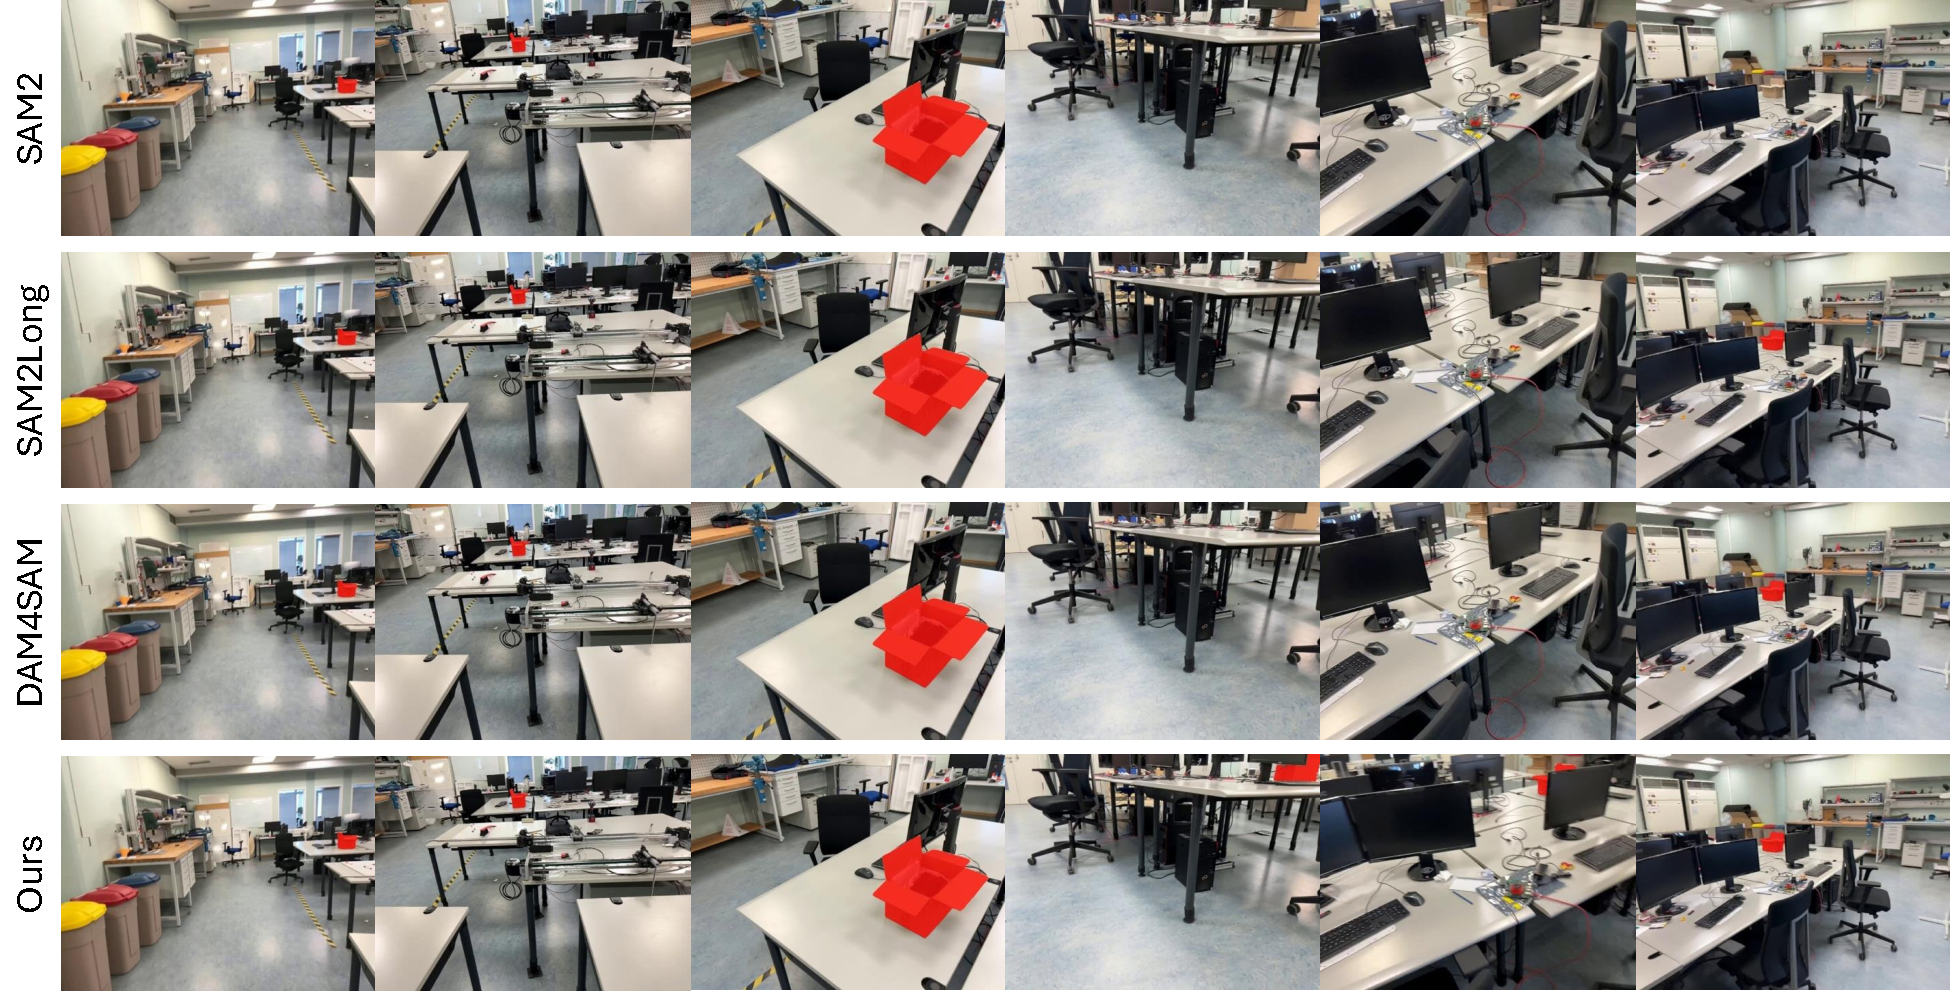
\includegraphics[width=1.0\textwidth]{figs/vis_comp.pdf}
    \vspace{-6mm}
    \caption{
    \textbf{Visual comparison of VOS methods.} The leftmost frame is used as the conditioned frame and provides the reference mask.
    }
    \label{fig:vis_comp}
\end{figure*}

The results are shown in \cref{tab:scannetpp-2d}, and we provide visualization at \cref{fig:vis_comp}.
On the ScanNet++ dataset, we further evaluate performance on a \emph{Selected Subset} specifically constructed to emphasize object reappearance.  
For each object track, we count the number of non-continuous visible segments, 
where a segment is defined as any contiguous span of visible frames whose length $\ell$ exceeds a minimal threshold $\ell_{\min}$.
Objects with frequent reappearance are typically associated with large viewpoint changes, since each disappearance–reappearance cycle often corresponds to observing the object from a substantially different angle or position.  
This subset, therefore, provides a focused evaluation of robustness under severe pose variation.

3AM achieves the best performance on both the \emph{Whole Set} (IoU 0.8898, highest Recall and Accuracy) and the challenging \emph{Selected Subset} (IoU 0.9061, Recall 0.7168, Accuracy 0.7737), highlighting its ability to maintain object identity even when the object reappears under large changes in viewpoint and spatial configuration. With a simple fallback mechanism, it also retains competitive results on conventional VOS benchmarks~\cite{perazzi2017davis, fan2019lasot, videnovic2025distractor} as shown in \cref{tab:scannetpp-2d}.

\vspace{-1em}
\subsubsection{Two-view Matching Comparison with SegMASt3R.}
We further compare our 3AM with SegMASt3R~\cite{Jayanti2025SegMASt3R}, a two-view matching approach built on MASt3R that associates segment masks between two images under large viewpoint changes, in \cref{tab:two_view_comparison}. SegMASt3R is not directly prompable and does not natively support $>2$ multiview tracking. Nevertheless, we include it as a strong two-view baseline by adopting the following protocol: we use the ground-truth initial mask as the source-frame candidate, and for each subsequent frame, we independently perform two-view mask matching against the source frame. To fairly compare the two approaches, when tracking with our 3AM, we don't use any memory other than the source frame.

Under this protocol, 3AM achieves \textbf{IoU} of $0.8915$, \textbf{Tracking Recall} of $0.5115$, and \textbf{Accuracy} of $0.6405$, whereas SegMASt3R obtains $0.6800$, $0.3628$, and $0.4053$, respectively. These results demonstrate 3AM not only provides stronger functionality, but also outperforms SegMASt3R even when restricted to two-view matching.

\begin{table}[t]
\centering
\setlength{\tabcolsep}{2mm}
\vspace{-3mm}
\begin{minipage}{0.48\textwidth}
\centering
\caption{{Quantitative comparison of two-view matching between 3AM and SegMASt3R on ScanNet++ Whole Set.}}
\label{tab:two_view_comparison}
\vspace{-3mm}
\resizebox{\textwidth}{!}{
\begin{tabular}{lccc}
\toprule
Method & IoU $\uparrow$ & {Tracking Recall} $\uparrow$ & Accuracy $\uparrow$\\
\midrule
SegMASt3R~\cite{Jayanti2025SegMASt3R} & 0.6800 & 0.3628 & 0.4053 \\
\rowcolor{black!10}
3AM (Ours) & \textbf{0.8915} & \textbf{0.5115} & \textbf{0.6405} \\
\bottomrule
\end{tabular}
}
\end{minipage}
\begin{minipage}{0.48\textwidth}

\centering
\caption{{Video Object Segmentation results on the Replica\cite{replica19arxiv} dataset.}}
\label{tab:replica-3d}
\vspace{-3mm}
\resizebox{\textwidth}{!}{
\begin{tabular}{lccc}
\toprule
Method & IoU $\uparrow$ & Tracking Recall $\uparrow$ & Accuracy $\uparrow$ \\
\midrule
SAM2~\cite{ravi2024sam2} & 0.4424 & 0.1432 & 0.2188 \\
SAM2Long~\cite{ding2024sam2long} & \cellcolor{yellow!25}0.7691 & \cellcolor{orange!25}0.5195 & \cellcolor{orange!25}0.6273 \\
DAM4SAM~\cite{videnovic2025distractor} & \cellcolor{orange!25}0.7744 & \cellcolor{yellow!25}0.5135 & \cellcolor{yellow!25}0.6124 \\
3AM (Ours) & \cellcolor{red!25}0.8119 & \cellcolor{red!25}0.6381 &  \cellcolor{red!25}0.6793 \\
\bottomrule
\end{tabular}
}
\end{minipage}

\vspace{-3mm}
\end{table}


\vspace{-1em}
\subsubsection{Replica.}

On the Replica dataset, 3AM achieves the best performance across all metrics (\cref{tab:replica-3d}), reaching an IoU of 0.8119 and surpassing SAM2 (0.4424), SAM2Long (0.7691), and DAM4SAM (0.7744). It also attains the highest Tracking Recall (0.6381) and Accuracy (0.6793), demonstrating robust tracking under the large viewpoint variations characteristic of Replica.

These results demonstrate that 3AM consistently surpasses prior methods and is particularly effective in scenarios involving object reappearance and large viewpoint variation, despite not relying on the explicit memory-selection mechanisms used in previous approaches. Due to space limitations, more visualization is provided in the supplementary materials.


\vspace{-0.5em}
\subsection{3D Evaluation}
\vspace{-0.5em}

We next evaluate our method on a 3D task.  
We adopt the class-agnostic 3D instance segmentation setting of ScanNet200, as it directly reflects a model’s ability to produce object-consistent predictions in 3D scenes.  
Prior approaches typically require explicit 3D fusion\cite{xu2024esam} or merging\cite{yang2023sam3d}, regardless of whether the proposals originate from 2D masks\cite{jung2025details} or 3D detectors\cite{boudjoghra2025openyolo, nguyen2024open3dis}.
Our goal is to demonstrate that this additional 3D-space merging is unnecessary: if 2D tracking is geometrically consistent across views, then reliable 3D instances can be obtained simply by projecting the tracked 2D masks into 3D.

Concretely, we follow prior methods\cite{zhao2025sam2object} and generate 2D proposals from SAM2 on keyframes selected by a stride-based sampling.  
These proposals are then propagated with 3AM, whose improved cross-view consistency enables stable object identification across multiple camera viewpoints.  
We perform merging using IoU and inter-mask precision to associate proposals over time, and project the resulting 2D tracks into 3D.  
In contrast, previous SAM2-based methods\cite{zhao2025sam2object} rely heavily on 3D merging because their tracking often drifts or fails under large viewpoint changes.  
Further implementation details are provided in the supplementary material.

As shown in Table~\ref{tab:scannet200-class-agnostic}, 3AM achieves the highest performance among online methods, with an AP of 47.3 and strong AP$_{50}$ and AP$_{25}$ scores (59.7 and 75.3).    
These results highlight a central finding of our work: robust 3D instance segmentation can emerge from geometry-aware tracking without heavy 3D supervision.



\begin{table}[t]
\centering
\small
\setlength{\tabcolsep}{2mm}
\vspace{-3mm}
\caption{\textbf{Class-agnostic 3D instance segmentation results of different methods on ScanNet200 dataset.}}
\label{tab:scannet200-class-agnostic}
\vspace{-3mm}
% \resizebox{\columnwidth}{!}{
\begin{tabular}{lccccc}
\toprule
Method & Type & 3D GT & AP $\uparrow$ & AP$_{50}$ $\uparrow$ & AP$_{25}$ $\uparrow$ \\
\midrule
SAMPro3D~\cite{xu2025sampro3d} & Offline & Yes & 18.0 & 32.8 & 56.1 \\
Open3DIS~\cite{nguyen2024open3dis} & Offline & Yes & \cellcolor{yellow!25}34.6 & 43.1 & 48.5 \\
SAI3D~\cite{yin2024sai3d} & Offline & Yes & 28.2 & 47.2 & 67.9 \\
SAM2Object~\cite{zhao2025sam2object} & Offline & Yes & 34.0 & \cellcolor{yellow!25}52.7 & \cellcolor{yellow!25}70.3 \\
\midrule
SAM3D~\cite{yang2023sam3d} & Online & Yes & 20.2 & 35.7 & 55.5 \\
ESAM~\cite{xu2024esam} & Online & Yes & \cellcolor{orange!25}42.2 & \cellcolor{red!25}63.7 & \cellcolor{red!25}79.6 \\
\midrule
3AM (Ours) & Online & No & \cellcolor{red!25}47.3 & \cellcolor{orange!25}59.7 & \cellcolor{orange!25}75.3 \\
\bottomrule
\end{tabular}
% }
\vspace{-3mm}
\end{table}


\vspace{-0.5em}
\subsection{Ablation Study}
\vspace{-0.5em}

\subsubsection{Component Analysis.}
We provide ablation studies in \cref{tab:component-eval} for Feature Source, Feature Merger Architecture, and Sampling Strategy.
We evaluate variants using MUSt3R or SAM2 features alone under the same training protocol to demonstrate that both features are necessary. MUSt3R provides geometric grounding, while SAM2 captures appearance correspondence. Without MUSt3R, relying solely on appearance matching from SAM2 introduces ambiguity and leads to degraded performance. One thing to note is that SAM2 performs worse after finetuning. We attribute this degradation to the absence of grounding information from MUSt3R, which causes the memory attention to be mistrained due to insufficient reference cues for distinguishing different objects.
Regarding the sampling strategy, naively applying random sampling results in worse performance than continuous sampling. When valid masks exist in both views, enforcing associations across large spatial discrepancies introduces ambiguity and leads to slower convergence.

\begin{table*}[t]
\centering
\setlength{\tabcolsep}{2mm}
\caption{\textbf{Component analysis on ScanNet++ selected subset.}}
\label{tab:component-eval}
\vspace{-3mm}
\resizebox{\textwidth}{!}{%
\begin{tabular}{cccccc}
\toprule
Feature Source & Feature Merger & Sampling Strategy & IoU & Tracking Recall & Accuracy \\
\midrule
SAM2 \& MUSt3R & Addition \& Convolution & FoV Sampling & 0.8771 & 0.6481 & 0.7149\\
SAM2 \& MUSt3R & Concatentation \& Attention & FoV Sampling & 0.8831 & 0.6744 & 0.7462\\
SAM2 \& MUSt3R & Hierarchical Cross Attention (Final) & Continuous Sampling & 0.7925 & 0.6518 & 0.7513\\
SAM2 \& MUSt3R & Hierarchical Cross Attention (Final) & Random Sampling & 0.7363 & 0.5371 & 0.6311 \\
MUSt3R  & - & FoV Sampling & 0.8461 & 0.5471 & 0.4129 \\
SAM2 & - & FoV Sampling & 0.6628 & 0.0038 & 0.0276 \\
SAM2 \& MUSt3R & Hierarchical Cross Attention (Final) & FoV Sampling & 0.9061 & 0.7168 & 0.7737\\
\bottomrule
\end{tabular}
}
% \vspace{-3mm}
\end{table*}

\vspace{-1em}
\subsubsection{Memory Selection.}
\label{subsubsec-memory-select}

\begin{table}[t]
\centering
\small
\setlength{\tabcolsep}{2mm}
\vspace{-3mm}

\begin{minipage}{0.48\textwidth}
\caption{Comparison of different memory selection methods on ScanNet++ Whole Set.}
\label{tab:memory-selection}
\vspace{-3mm}
\resizebox{\textwidth}{!}{
\begin{tabular}{lccc}
\toprule
Method & IoU $\uparrow$ & Tracking Recall $\uparrow$ & Accuracy $\uparrow$ \\
\midrule
3AM & \cellcolor{yellow!25}0.8898 & \cellcolor{yellow!25}0.5630 & \cellcolor{yellow!25}0.7155 \\
DAM4SAM-3AM~\cite{videnovic2025distractor} & \cellcolor{orange!25}0.8941 & \cellcolor{orange!25}0.5471 &  \cellcolor{orange!25}0.7204 \\
SAM2Long-3AM~\cite{ding2024sam2long} & \cellcolor{red!25}0.9004 & \cellcolor{red!25}0.5498 & \cellcolor{red!25}0.7361 \\
\bottomrule
\end{tabular}
}
\end{minipage}
\begin{minipage}{0.48\textwidth}
\caption{Comparison of different 3D reconstruction backbones.}
\label{tab:3D_backbone}
\resizebox{\textwidth}{!}{
\begin{tabular}{lccc}
\toprule
\textbf{Model} & \textbf{Online} & \textbf{Frame Num} & \textbf{ScanNet++ Selected Subset Tracking Recall} \\
\midrule
VGGT & $\times$ & $\sim$200       & --      \\
$\pi^3$ & $\times$ & $\sim$300    & --      \\
CUT3R & \checkmark & $>10{,}000$  &  0.2751 \\
\rowcolor{black!10}
MUSt3R & \checkmark & $>10{,}000$  &  \textbf{0.7168}  \\
\bottomrule
\end{tabular}
}
\end{minipage}
\vspace{-3mm}
\end{table}

We further analyze the role of memory selection by combining 3AM with existing strategies proposed for SAM2.  
Table~\ref{tab:memory-selection} reports results on the ScanNet++ Whole Set.  
3AM, which uses the original SAM2 memory-selection mechanism, already achieves strong performance with an IoU of 0.8898.  
When we incorporate alternative memory-selection policies, such as those from DAM4SAM~\cite{videnovic2025distractor} or SAM2Long~\cite{ding2024sam2long}, we observe modest improvements: DAM4SAM-3AM slightly increases Accuracy to 0.7204, while SAM2Long-3AM achieves the highest IoU (0.9004) and Accuracy (0.7361).
These results suggest that 3AM already delivers strong and stable performance without relying on specialized memory-selection policies.  
While alternative strategies such as those from SAM2Long or DAM4SAM offer small additional gains, their impact is relatively limited compared to the improvements brought by 3AM itself.  
We view the design of memory-selection mechanisms tailored specifically for 3AM as an interesting direction for future work.

\vspace{-1em}
\subsubsection{3D Foundataion Models.}
\label{subsubsec-3d-models}

\begin{figure}[t]
    \centering
    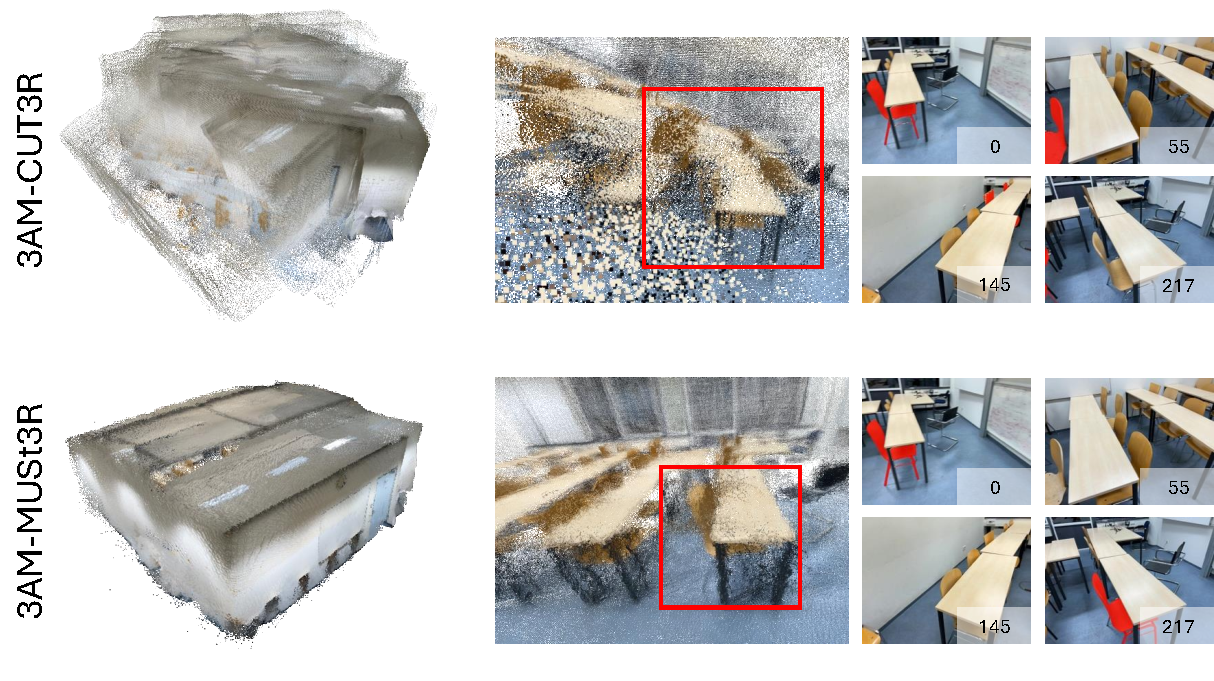
\includegraphics[width=1.0\linewidth]{figs/vis_cut3r.pdf}
    \vspace{-6mm}
    \caption{
    \textbf{Visual comparison of different 3D reconstruction backbones.} (\emph{Top}) CUT3R's reconstruction lacks stable object alignment; the same table appears at inconsistent 3D locations. Such geometric instability weakens feature distinctiveness, making reliable tracking difficult. (\emph{Bottom}) In contrast, MUSt3R provides coherent and stable object alignment across viewpoints, yielding features that preserve object identity and enable robust tracking
    % \textbf{Visual comparison of different 3D reconstruction backbones used for feature extraction.}  
    % The top row shows the geometry produced by CUT3R, whose reconstruction lacks stable object alignment, i.e., the same table appears at inconsistent 3D locations.  
    % Since our method relies on backbone features to establish cross-view correspondence, such geometric instability weakens the distinctiveness and consistency of the extracted features, making reliable tracking difficult.  
    % In contrast, MUSt3R (bottom row) provides much more coherent and stable object alignment across viewpoints, yielding feature representations that preserve object identity under large pose changes and enabling significantly more robust tracking.
    }
    \label{fig:comp_3r}
\end{figure}

We compare 3D foundation models in Table~\ref{tab:3D_backbone}. VGGT and $\pi^3$ operate offline on frame batches, unsuitable for online tracking. CUT3R supports online operation, but yields limited instance-level alignment as shown in \cref{fig:comp_3r}, reflected by its Tracking Recall of 0.2751 on the ScanNet++ Selected Subset. MUSt3R is fully online with substantially stronger object alignment across viewpoints. This alignment is essential: consistent 3D alignment enables stable 2D cross-view correspondence, allowing reliable mask propagation without explicit 3D merging.

% To understand the impact of different 3D reconstruction backbones, we compare several recent 3D foundation models in Table~\ref{tab:3D_backbone}.  
% VGGT and $\pi^3$ are offline models that operate on frame batches and therefore cannot be used in an online tracking pipeline.  
% CUT3R supports online operation but yields limited instance-level alignment as shown in \cref{fig:comp_3r}, reflected by its Tracking Recall of 0.2751 on the ScanNet++ Selected Subset.
% In contrast, MUSt3R is fully online and produces substantially stronger object-level alignment across viewpoints.  
% We argue that such alignment is essential for our task: consistent alignment in 3D directly supports stable cross-view correspondence in 2D, enabling reliable mask propagation without the need for explicit 3D-space merging.

% More ablation studies are provided in the supplementary materials.